\documentclass{report}
\usepackage{amsmath, amssymb, amsthm}
\usepackage{algorithm, algorithmic}
\usepackage{graphicx}
\usepackage{xcolor}
\usepackage{algorithm}      % Para el entorno algorithm
\usepackage{algpseudocode} % Para el entorno algorithmic
\usepackage{amsthm}
\usepackage{algorithmic} 

\newtheorem{theorem}{Teorema} % Define el entorno "theorem"

\title{Diseño y Análisis de Algortimos para el problema Gestión Agrícola}
\author{Amanda Cordero Lezcano\\Christopher Guerra Herrero}
\date{}

\begin{document}
	
	\maketitle
	\tableofcontents
	
	\chapter{Problema de Gestión Agrícola}
	
	
	La gestión agrícola moderna enfrenta desafíos críticos relacionados con la optimización de recursos, tanto en la planificación de cultivos como en la asignación eficiente de mano de obra. Estos problemas requieren enfoques algorítmicos robustos para maximizar beneficios económicos y minimizar tiempos de ejecución, asegurando un uso sostenible de los recursos disponibles. En este capítulo, se formalizan dos problemas centrales en este contexto y se establece su relación con problemas clásicos de optimización combinatoria.

	\section{Rotación de Cultivos con Ventanas Temporales}
	Se desea seleccionar cultivos para sembrar en un período determinado, considerando:
	\begin{itemize}
		\item \textbf{Prioridad económica}: Cada cultivo genera un beneficio monetario asociado.
		\item \textbf{Tiempo de ocupación}: Período durante el cual la tierra está ocupada (desde la siembra hasta la cosecha).
		\item \textbf{Ventana temporal fija}: Duración total disponible para la siembra.
	\end{itemize}
	
	\textbf{Objetivo}: Seleccionar un conjunto de cultivos (con posibles repeticiones) que maximice el beneficio total sin exceder la ventana temporal. Este problema es equivalente al \textbf{Problema de la Mochila Ilimitada (Unbounded Knapsack)}, donde:
	\begin{itemize}
		\item \textit{Peso del elemento} $\equiv$ Tiempo de ocupación del cultivo.
		\item \textit{Valor del elemento} $\equiv$ Beneficio económico del cultivo.
		\item \textit{Capacidad de la mochila} $\equiv$ Ventana temporal disponible.
	\end{itemize}
	
	\section{Asignación de Tareas}
	Se debe distribuir un conjunto de tareas agrícolas (ej: podar, regar, cosechar) entre un grupo de obreros, considerando:
	\begin{itemize}
		\item \textbf{Tiempo de ejecución}: Cada tarea requiere un tiempo específico.
		\item \textbf{Recursos limitados}: Número fijo de obreros disponibles.
	\end{itemize}
	
	\textbf{Objetivo}: Asignar tareas a obreros minimizando el tiempo total de ejecución (\textit{makespan}). Este problema se modela como \textbf{Balanceo de Carga (Load Balancing)} en sistemas distribuidos.
	
	
	\chapter{Problema Unbounded Knapsack}
El problema \textbf{Unbounded Knapsack (UK)} es una extensión del clásico problema de la mochila (\textbf{Knapsack (K)}), donde los elementos pueden ser seleccionados múltiples veces. Este problema tiene aplicaciones en diversas áreas, como la logística, la planificación de recursos y la optimización de inventarios. En este texto, exploraremos la relación entre \textbf{UK} y \textbf{K}, y demostraremos que \textbf{UK} es un problema NP-duro mediante una reducción formal desde \textbf{UK} a \textbf{K}.

\section{Demostración de que Unbounded Knapsack es NP-duro}

Para demostrar que el problema \textbf{Unbounded Knapsack (UK)} es NP-duro, realizaremos una reducción desde \textbf{UK} a \textbf{Knapsack (K)}, que es un problema NP-completo. La idea central es transformar una instancia de \textbf{UK} en una instancia equivalente de \textbf{K}, resolviendo subproblemas de manera iterativa hasta obtener una solución completa.

\subsection*{Definición del problema UK}

Dada una instancia de \textbf{UK}, se tiene:
\begin{itemize}
	\item Un conjunto de \( n \) elementos, donde cada elemento \( i \) tiene un peso \( w_i \) y un valor \( v_i \).
	\item Una capacidad máxima de la mochila \( W \).
\end{itemize}

El objetivo es maximizar el valor total de los elementos seleccionados sin exceder la capacidad \( W \), permitiendo que cada elemento pueda ser seleccionado múltiples veces.

\subsection*{Reducción de UK a K}

La reducción se realiza mediante el algoritmo siguiente:


\begin{algorithm}[H]
	\label{uk_to_k}\caption{Reducción de UK a K}

	\State
	\State 1. \textbf{Inicialización:}
	\State \quad \( S \gets \emptyset \)  \Comment{Conjunto de elementos seleccionados}
	\State \quad \( P \gets 0 \)          \Comment{Peso total acumulado}
	\State \quad \( R \gets W \)          \Comment{Capacidad residual inicial}
	
	\State
	\State 2. \textbf{Iteración:}
	\While{\( R > 0 \)}
	\State \quad a. Resolver \textbf{UK} sobre el conjunto de elementos \( E \) con capacidad \( R \).
	\State \quad b. Sea \( S_{\text{temp}} \) el conjunto de elementos seleccionados (sin repeticiones) y \( P_{\text{temp}} \) el peso total de \( S_{\text{temp}} \).
	\If{\( S_{\text{temp}} = \emptyset \)}
	\State \quad \quad \textbf{Break}  \Comment{No se pueden agregar más elementos}
	\EndIf
	\State \quad c. Actualizar:
	\State \quad \quad \( S \gets S \cup S_{\text{temp}} \)
	\State \quad \quad \( P \gets P + P_{\text{temp}} \)
	\State \quad \quad \( R \gets R - P_{\text{temp}} \)
	\State \quad d. Eliminar los elementos de \( S_{\text{temp}} \) de \( E \): \( E \gets E \setminus S_{\text{temp}} \)
	\EndWhile
	
	\State
	\State 3. \textbf{Terminación:}
	\State \quad \textbf{Devolver} \( S \)  \Comment{Conjunto de elementos seleccionados}
\end{algorithm}

\subsection*{Demostración de correctitud}

Para demostrar que la reducción de \textbf{UK} a \textbf{K} es válida, debemos probar que la solución obtenida mediante el algoritmo descrito es equivalente a la solución óptima de \textbf{K}. A continuación, se detallan los aspectos clave de la demostración:

\begin{itemize}
	\item \textbf{No repetición de elementos}: En cada iteración, el algoritmo selecciona un subconjunto de elementos \textbf{sin repeticiones}, es decir, cada elemento se incluye en la mochila a lo sumo una vez. Esto es consistente con la definición de \textbf{K}, donde los elementos no pueden repetirse.
	
	\item \textbf{Optimalidad}: Los elementos sin repetición de cada iteración de UK son parte de la solución óptima de K ya que si alguno no lo fuera es porque este puede ser remplazado por otro u otros que en total maximizen la ganancia, pero en tal caso UK los hubiera seleccionados.
	
	\item \textbf{Conjunto finito de elementos}: Dado que el conjunto de elementos es finito, el algoritmo termina en un número finito de pasos. En cada iteración, se elimina al menos un elemento del conjunto de candidatos, lo que garantiza que el proceso no continúe indefinidamente.
	
	\item \textbf{Complejidad de la transformación}: La reducción realiza una transformación en tiempo polinomial. En el peor caso, el algoritmo ejecuta \textbf{UK} una vez por cada elemento distinto, lo que resulta en una complejidad de \( O(n \cdot T_{\text{UK}}) \), donde \( T_{\text{UK}} \) es la complejidad de resolver \textbf{UK}. Si \textbf{UK} fuera resoluble en tiempo polinomial, entonces \textbf{K} también lo sería, ya que la transformación preserva la clase de complejidad.
	
	\item \textbf{Uso completo de la capacidad}: El algoritmo termina cuando no se pueden agregar más elementos sin exceder la capacidad de la mochila. Esto asegura que la capacidad \( W \) se utiliza de manera óptima, y la solución acumulada es equivalente a la solución óptima de \textbf{K}.
\end{itemize}
Mediante esta reducción, hemos demostrado que cualquier instancia de \textbf{K} puede ser transformada en una secuencia de tamaño polinomial de instancias de \textbf{UK}. Dado que \textbf{K} es un problema NP-completo, concluimos que \textbf{UK} es NP-duro.

\section{Algoritmo exacto}

Ataquemos el problema con Programación dinámica. La idea de solución es similar a la vista en \cite{CLRS2009} para el problema 0/1 Knapsack.
Utilizamos un arreglo $\text{DP}$ donde $\text{DP}[i]$ almacena el valor máximo alcanzable con una mochila de capacidad $i$. Comenzamos con capacidad 0 y progresivamente resolvemos capacidades mayores usando soluciones ya calculadas.

\subsection*{Subestructura óptima}
La propiedad clave es que la solución óptima para capacidad $i$ puede construirse a partir de soluciones óptimas para capacidades menores. Si un elemento de peso $w_j$ se incluye en la solución óptima para capacidad $i$, entonces el valor óptimo será $v_j + \text{DP}[i - w_j]$.

%------------------------------------------
\subsection{Programación dinámica}
\subsubsection*{Estados y transiciones}
\begin{itemize}
    \item \textbf{Estado}: $\text{DP}[i]$ representa el valor máximo para capacidad $i$.
    \item \textbf{Inicialización}: $\text{DP}[0] = 0$ (ningún elemento cabe en capacidad 0).
    \item \textbf{Transición}: Para cada capacidad $i$ y elemento $j$:
        \[
        \text{DP}[i] = \max\left(\text{DP}[i],\, v_j + \text{DP}[i - w_j]\right) \quad \text{si } w_j \leq i
        \]
\end{itemize}

\begin{algorithm}[H]
	\caption{Pseudocódigo Unbounded Knapsack}
	\State{$W, \texttt{weights}, \texttt{values}$}
    \State Inicializar arreglo $\text{DP}[0 \dots W]$ con 0's
    \For{$i = 1$ to $W$}
        \For{$j = 0$ to $n-1$}
            \If{$\texttt{weights}[j] \leq i$}
                \State $\text{DP}[i] \gets \max(\text{DP}[i],\, \text{DP}[i - \texttt{weights}[j]] + \texttt{values}[j])$
            \EndIf
        \EndFor
    \EndFor
    \State \Return $\text{DP}[W]$
\EndProcedure
\end{algorithm}

\subsubsection*{Complejidad}
\begin{itemize}
    \item \textbf{Temporal}: $O(n \cdot W)$ (dos bucles anidados: $W$ iteraciones externas, $n$ internas).
    \item \textbf{Espacial}: $O(W)$ (solo se almacena un arreglo de tamaño $W+1$).
\end{itemize}

%------------------------------------------
\subsection{Análisis del algoritmo}
\subsubsection*{Correctitud}
La demostración se basa en inducción matemática:

\begin{itemize}
    \item \textbf{Caso base}: $\text{DP}[0] = 0$ es trivialmente correcto.
    
    \item \textbf{Hipótesis inductiva}: Supongamos que $\text{DP}[k]$ es óptimo para todo $k < i$.
    
    \item \textbf{Paso inductivo}: Para capacidad $i$, consideramos todos los elementos $j$ con $w_j \leq i$. Si el elemento $j$ es parte de la solución óptima, entonces:
    \[
    \text{DP}[i] = v_j + \text{DP}[i - w_j]
    \]
    Por hipótesis inductiva, $\text{DP}[i - w_j]$ ya es óptimo. Al maximizar sobre todos los $j$, garantizamos que $\text{DP}[i]$ también es óptimo.
\end{itemize}

El procesamiento en orden ascendente de capacidades asegura que al calcular $\text{DP}[i]$, todos los valores $\text{DP}[k]$ para $k < i$ ya han sido computados correctamente, permitiendo reutilizar soluciones previas.


\section{Algoritmo de aproximación}
Con información de \cite{Rhee2016}

Comencemos por describir un algoritmo que garantiza una solución dentro de un factor de 2 del valor óptimo. Supongamos que el artículo $ j $ tiene la mayor densidad de beneficio, definida como $ p_i / w_i $, donde $ p_i $ es el beneficio del artículo $ i $ y $ w_i $ es su peso. Denotamos $ z_L $ como el valor objetivo obtenido al seleccionar tantas unidades del artículo $ j $ como sea posible sin exceder la capacidad de la mochila $ C $. Formalmente:
\[
z_L = p_j \lfloor C / w_j \rfloor,
\]
donde $ \lfloor C / w_j \rfloor $ representa el número máximo de unidades enteras del artículo $ j $ que caben en la mochila.

Es importante notar que si se relaja la restricción de integridad (es decir, si se permite fraccionar los artículos), el valor objetivo óptimo sería:
\[
z = p_j (C / w_j),
\]
el cual constituye una cota superior para el valor óptimo $ z^* $ bajo las restricciones originales. Por lo tanto, se cumple que:
\[
z_L \leq z^* \leq z.
\]

Además, dado que $ z = z_L + p_j \epsilon $, donde $ 0 \leq \epsilon < 1 $, se deduce que:
\[
z \leq 2z_L.
\]

En consecuencia, tenemos que:
\[
z^* \leq 2z_L,
\]
lo cual implica que el algoritmo que selecciona únicamente el artículo con mayor densidad de beneficio y llena la mochila con este tipo de elementos constituye una $ 2 $-aproximación al valor óptimo del problema.

\section{Experimentación gráfica}

\begin{figure}[H]
	\centering
	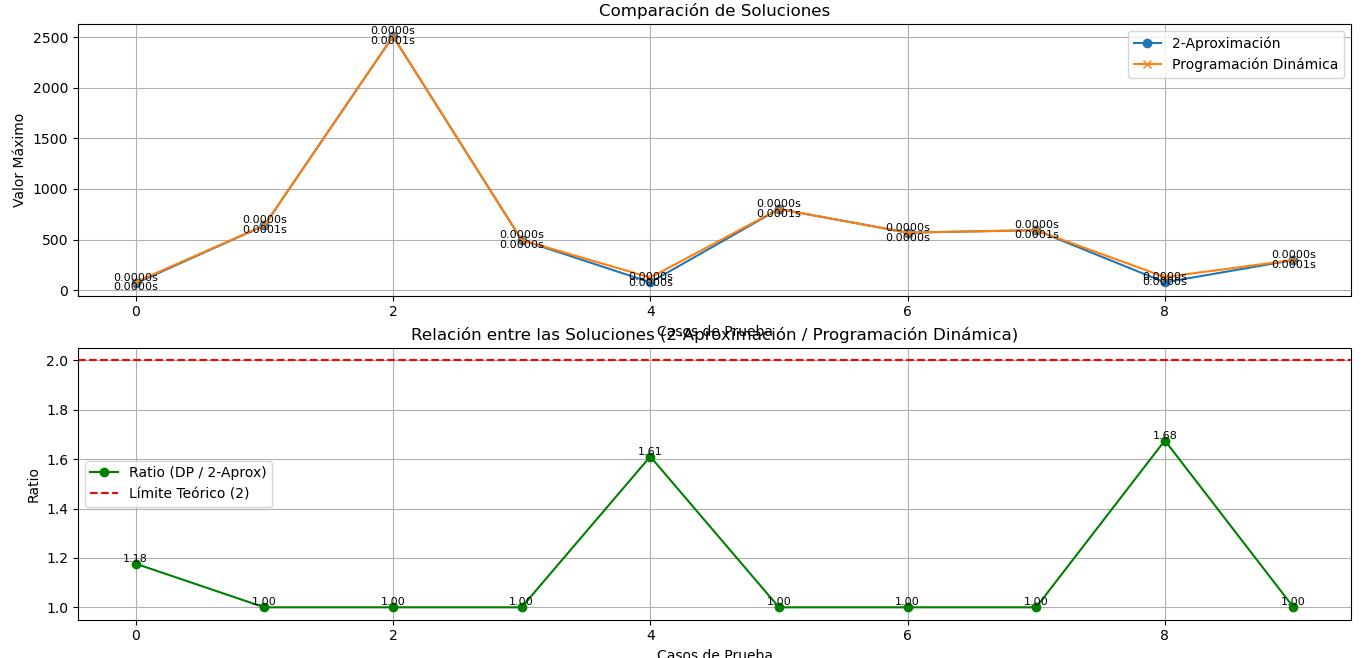
\includegraphics[width=1\linewidth]{Figure_2}
	\caption{Comparación gráfica entre los algoritmos}
	\label{fig:figure1}
\end{figure}

	\chapter{Problema Load Balancing}
	
	{Con información de \cite{Kleinberg2005} y \cite{Garey1979}\\\\}
	
	Formulamos el \textbf{Problema de Load Balancing} de la siguiente manera. Se nos da un conjunto de \( m \) máquinas \( M_1, \dots, M_m \) y un conjunto de \( n \) trabajos; cada trabajo \( j \) tiene un tiempo de procesamiento \( t_j \). Buscamos asignar cada trabajo a una de las máquinas de manera que las cargas colocadas en todas las máquinas estén lo más \textit{balanceadas} posible.
	
	Más concretamente, en cualquier asignación de trabajos a máquinas, podemos denotar por \( A(i) \) el conjunto de trabajos asignados a la máquina \( M_i \). Bajo esta asignación, la máquina \( M_i \) trabajará un tiempo total de
	\[
	T_i = \sum_{j \in A(i)} t_j,
	\]
	y declaramos que esta es la carga en la máquina \( M_i \). Buscamos minimizar una cantidad conocida como el \textit{makespan}, que es simplemente la carga máxima en cualquier máquina:
	\[
	T = \max_i T_i.
	\]
	


	Nuestro problema de optimización tiene una versión de decisión: Dado un valor $ M $, ¿existe una asignación de tareas tal que el makespan sea $ \leq M $?
	A continuación nos apoyaremos del problema de desición y del conocido problema Partition para demostrar que la versión de optimización de Load Balancing es NP duro.
	
	\section{Demostración de que Load Balancing es NP duro}
	
		
	Para demostrar que el problema de decisión es NP-completo, realizamos una reducción desde el problema \textbf{Partition}, primero demostremos que este es NP-completo reduciéndolo a Subset-Sum.
	
	\subsection{Demostración de que Partition es NP completo}
	
	Problema Partition:	Dado un conjunto de números $ \{p_1, p_2, \dots, p_n\} $, ¿es posible dividirlo en dos subconjuntos disjuntos $ A $ y $ B $ tales que:
	\[
	\sum_{p_i \in A} p_i = \sum_{p_i \in B} p_i?
	\]
	
	Sea $ P = \sum_{i=1}^n p_i $. El problema puede reformularse como: ¿existe una partición tal que:
	\[
	\sum_{p_i \in A} p_i = \frac{P}{2}?
	\]
	
	
	Para demostrar que \textbf{Partition} es NP-completo, seguimos los siguientes pasos:
	
	\subsubsection*{Paso 1: Partition está en NP}
	
	Un problema está en NP si, dada una solución candidata, podemos verificar su validez en tiempo polinomial.
	
	Una solución candidata para \textbf{Partition} consiste en un subconjunto $ A \subseteq S $. Para verificar si $ A $ es una solución válida:\\
	- Calculamos $ \text{suma}(A) = \sum_{x \in A} x $.\\
	- Verificamos si $ \text{suma}(A) = \frac{\sum_{i=1}^n a_i}{2} $.\\
	- Esto se puede hacer en tiempo polinomial con respecto al tamaño de $ S $.
	
	Por lo tanto, \textbf{Partition} está en NP.
	
	\subsubsection*{Paso 2: Partition es NP-duro}
	
	Para demostrar que \textbf{Partition} es NP-duro, realizamos una reducción polinomial desde el problema \textbf{Subset-Sum}, que es conocido como NP-completo.
	
	\subsubsection*{Problema Subset-Sum}
	
	El problema \textbf{Subset-Sum} se define como sigue:
	
	\textbf{Entrada}: Un conjunto finito $ S = \{a_1, a_2, \dots, a_n\} $ de números enteros positivos y un objetivo $ T $.
	
	\textbf{Pregunta}: ¿Existe un subconjunto $ A \subseteq S $ tal que:
	\[
	\sum_{x \in A} x = T?
	\]
	
	\subsubsection*{Reducción desde Subset-Sum a Partition}
	
	Dada una instancia del problema \textbf{Subset-Sum} con conjunto $ S = \{a_1, a_2, \dots, a_n\} $ y objetivo $ T $, construimos una instancia del problema \textbf{Partition} como sigue:
	
	1. Calcula la suma total de los elementos de $ S $:
	\[
	P = \sum_{i=1}^n a_i.
	\]
	
	2. Agrega un nuevo número $ b $ al conjunto $ S $, donde:
	\[
	b = |P - 2T|.
	\]
	
	3. Define el nuevo conjunto $ S' = S \cup \{b\} $.
	
	Ahora preguntamos: ¿Es posible particionar $ S' $ en dos subconjuntos $ A $ y $ B $ tales que:
	\[
	\sum_{x \in A} x = \sum_{y \in B} y?
	\]
	
	En tal caso la cardinalidad de los subconjuntos será $$\frac{P + |P - 2T|}{2}$$ Por lo que uno de los dos tendrá $T$ de cardinalidad al excluir a $b$
	
	
	
	
	\subsection*{Reducción desde Parition a Load Balancing}
	Dada una instancia del problema Load Balancing de decisión, construimos el problema Partition como sigue:
	\begin{itemize}
		\item Sea $ m = 2 $ (dos máquinas).
		\item Asigna los tiempos de procesamiento $ p_1, p_2, \dots, p_n $ a las tareas.
		\item Define $ T = \frac{P}{2} $.
	\end{itemize}
	
	Ahora preguntamos: ¿Existe una asignación de tareas a las dos máquinas tal que el makespan sea $ \leq T $?
	
	\subsubsection*{Equivalencia}
	Si existe una asignación de tareas entonces habrá una partición. Si no existe, no existirá la partición. Por lo tanto, resolver el problema de decisión de Load Balancing permite resolver el problema Partition.
	Como el problema Partition es NP-completo y hemos mostrado que cualquier instancia de Partition puede reducirse en tiempo polinomial a una instancia del problema de decisión de Load Balancing, y la solución de este es verificable en tiempo polinomial de forma trivial (pertenece a NP), concluimos que el problema de decisión de Load Balancing es NP-completo.
	
	
	Finalmente, demostramos que el problema de optimización de Load Balancing es NP-duro. Para ello, notamos que:
	
	1. Si podemos resolver el problema de optimización (encontrar el makespan mínimo $ T^* $), entonces podemos resolver el problema de decisión para cualquier valor $ T $ comparando $ T $ con $ T^* $:
	\[
	\text{Respuesta al problema de decisión} =
	\begin{cases}
		\text{sí}, & \text{si } T \geq T^*, \\
		\text{no}, & \text{si } T < T^*.
	\end{cases}
	\]
	
	2. Como el problema de decisión es NP-completo, resolver el problema de optimización implica resolver un problema NP-completo.
	
	Por lo tanto, el problema de optimización de Load Balancing es NP-duro.
	
		\section{Algortimo Exacto}
		Búsqueda con Backtracking y Poda es una alternativa para resolver el problema de Load Balancing, aunque su escalabilidad está limitada por la complejidad computacional del problema.

		Esta técnica explora sistemáticamente todas las posibles asignaciones de trabajos a máquinas, pero utiliza estrategias de poda para eliminar ramas del árbol de búsqueda que no pueden conducir a una solución mejor que la ya encontrada.

		\subsection*{Pasos Clave}

		\textbf{1. Ordenar Trabajos}
		\begin{itemize}
			\item Ordenar los trabajos en orden descendente de \( t_j \). 
			\item \textbf{Propósito}: Asignar primero los trabajos más grandes para revelar rápidamente soluciones subóptimas y permitir una poda temprana.
		\end{itemize}

		\textbf{2. Inicializar Variables}
		\begin{itemize}
			\item Mantener dos registros fundamentales:
			\begin{enumerate}
				\item \( T_{\text{best}} \): El mejor makespan encontrado hasta el momento (inicializado con una cota superior, como la suma total de \( t_j \)).
				\item \( \text{cargas} = [c_1, c_2, \dots, c_m] \): Arreglo que almacena la carga parcial de cada máquina \( M_i \) (inicializado en 0).
			\end{enumerate}
		\end{itemize}

		\textbf{3. Exploración Recursiva}
		\begin{itemize}
			\item Para cada trabajo \( j \) (en orden descendente):
			\begin{enumerate}
				\item Asignar \( j \) a cada máquina \( M_i \).
				\item Actualizar la carga parcial de \( M_i \): \( c_i \leftarrow c_i + t_j \).
				\item Si en cualquier momento \( c_i \geq T_{\text{best}} \), detener la exploración de esa rama (\textbf{poda por optimalidad}).
				\item Llamar recursivamente al algoritmo para el siguiente trabajo \( j+1 \).
				\item Deshacer la asignación (\( c_i \leftarrow c_i - t_j \)) para probar otras máquinas (\textbf{backtracking}).
			\end{enumerate}
		\end{itemize}

		\textbf{4. Estrategias de Poda}
		\begin{itemize}
			\item \textbf{Poda por Carga Parcial}: Si \( c_i > T_{\text{best}} \), ignorar asignaciones futuras a \( M_i \).
			\item \textbf{Cota Inferior}: Calcular una cota inferior para el makespan parcial usando:
			\[
			T_{\text{min}} = \max\left( \max_{1 \leq i \leq m} c_i,\; \frac{1}{m} \left( \sum_{i=1}^m c_i + \sum_{j=k}^n t_j \right) \right)
			\]
			donde \( k \) es el índice del trabajo actual. Si \( T_{\text{min}} \geq T_{\text{best}} \), podar la rama.
		\end{itemize}

		\subsection*{Complejidad Temporal}
		$O(m^n)$ en el peor caso

		\begin{algorithm}[H]
			\caption{Backtracking con Poda para Load Balancing}

			\Require Lista de trabajos $jobs$, número de máquinas $m$
			\Ensure Makespan mínimo $T_{\text{best}}$
			
			\State Ordenar $jobs$ en orden descendente de $t_j$ \Comment{$t_1 \geq t_2 \geq \dots \geq t_n$}
			\State Inicializar $T_{\text{best}} \leftarrow \sum_{j=1}^n t_j$ \Comment{Cota superior inicial}
			\State Inicializar cargas $loads \leftarrow [0, 0, \dots, 0]$ \Comment{Vector de tamaño $m$}
			
			\Function{Backtrack}{$current\_job$, $loads$, $T_{\text{best}}$}
				\If{$current\_job = n$}
					\State \Return $\max(loads)$ \Comment{Base case: todos los trabajos asignados}
				\EndIf
				
				\State $job \leftarrow jobs[current\_job]$
				\For{$i \leftarrow 1$ \textbf{to} $m$}
					\If{$loads[i] + job \geq T_{\text{best}}$}
						\State \Continue \Comment{Poda: rama no prometedora}
					\EndIf
					
					\State $loads[i] \leftarrow loads[i] + job$ \Comment{Asignar trabajo a máquina $i$}
					\State $new\_T \leftarrow \Call{Backtrack}{current\_job + 1, loads, T_{\text{best}}}$
					
					\If{$new\_T < T_{\text{best}}$}
						\State $T_{\text{best}} \leftarrow new\_T$ \Comment{Actualizar mejor solución}
					\EndIf
					
					\State $loads[i] \leftarrow loads[i] - job$ \Comment{Backtracking: deshacer asignación}
				\EndFor
				\State \Return $T_{\text{best}}$
			\EndFunction
			
			\State \Return $\Call{Backtrack}{0, loads, T_{\text{best}}}$ \Comment{Llamada inicial}

			\end{algorithm}
		
			\section{Algoritmos de aproximación}

	Hemos demostrado que el problema de Load Balancing (en su versión de optimización) es NP-duro mediante una reducción desde el problema Partition al problema de decisión, y luego conectando el problema de decisión con el problema de optimización. Ahora vamos a ver algunos algoritmos para aproximar la solución del mismo.
	



	
	\subsection*{Greedy-Balance}
	
	Primero consideramos un algoritmo greedy muy simple para el problema. El algoritmo hace un recorrido por los trabajos en cualquier orden; cuando llega al trabajo \( j \), lo asigna a la máquina cuya carga sea la más pequeña hasta ese momento.
	

\begin{algorithm}[H]
	\caption{Greedy-Balance}
	\label{alg:greedy-balance}
		\State Empezar sin trabajos asignados
		\For{cada máquina \( M_i \)}
		\State \( T_i \gets 0 \) \Comment{Inicializar la carga de la máquina}
		\State \( A(i) \gets \emptyset \) \Comment{Inicializar el conjunto de trabajos asignados a \( M_i \)}
		\EndFor
		
		\For{cada trabajo \( j = 1, \dots, n \)}
		\State Sea \( M_i \) la máquina con la menor carga
		\State Asignar el trabajo \( j \) a la máquina \( M_i \)
		\State \( A(i) \gets A(i) \cup \{j\} \)
		\State \( T_i \gets T_i + t_j \)
		\EndFor
\end{algorithm}

	
	\subsection*{Análisis del Algoritmo}
	
	Sea \( T \) el makespan de la asignación resultante; queremos mostrar que \( T \) no es mucho mayor que el makespan mínimo posible \( T^* \). Por supuesto, al intentar hacer esto, nos encontramos inmediatamente con el problema básico mencionado anteriormente: necesitamos comparar nuestra solución con el valor óptimo \( T^* \), aunque no sabemos cuál es este valor y no tenemos forma de calcularlo. Para el análisis, por lo tanto, necesitaremos una cota inferior para el óptimo, una cantidad con la garantía de que, no importa cuán bueno sea el óptimo, no puede ser menor que esta cota.
	
	Hay muchas posibles cotas inferiores para el óptimo. Una idea para una cota inferior se basa en considerar el tiempo total de procesamiento \( \sum_j t_j \). Una de las \( m \) máquinas debe hacer al menos una fracción \( 1/m \) del trabajo total, y por lo tanto tenemos lo siguiente:
	
	\begin{equation} \label{eq:lower-bound-1}
		T^* \geq \frac{1}{m} \sum_j t_j.
	\end{equation}
	
	Hay un tipo particular de caso en el que esta cota inferior es demasiado débil para ser útil. Supongamos que tenemos un trabajo que es extremadamente largo en relación con la suma de todos los tiempos de procesamiento. En una versión suficientemente extrema de esto, la solución óptima colocará este trabajo en una máquina por sí solo, y será el último en terminar. En tal caso, nuestro algoritmo greedy en realidad produciría la solución óptima, pero la cota inferior en (\ref{eq:lower-bound-1}) no es lo suficientemente fuerte para establecer esto.
	
	Esto sugiere la siguiente cota inferior adicional para \( T^* \):
	
	\begin{equation} \label{eq:lower-bound-2}
		T^* \geq \max_j t_j.
	\end{equation}
	
	Ahora estamos listos para evaluar la asignación obtenida por nuestro algoritmo greedy.

		El algoritmo \textbf{Greedy-Balance} produce una asignación de trabajos a máquinas con un makespan \( T \leq 2T^* \).
	
		Aquí está el plan general para la demostración. Al analizar un algoritmo de aproximación, se compara la solución obtenida con lo que se sabe sobre el óptimo; en este caso, nuestras cotas inferiores (\ref{eq:lower-bound-1}) y (\ref{eq:lower-bound-2}). Consideramos una máquina \( M_i \) que alcanza la carga máxima \( T \) en nuestra asignación, y nos preguntamos: ¿Cuál fue el último trabajo \( j \) asignado a \( M_i \)? Si \( t_j \) no es demasiado grande en relación con la mayoría de los otros trabajos, entonces no estamos muy por encima de la cota inferior (\ref{eq:lower-bound-1}). Y, si \( t_j \) es un trabajo muy grande, entonces podemos usar (\ref{eq:lower-bound-2}).
		
		Cuando asignamos el trabajo \( j \) a \( M_i \), la máquina \( M_i \) tenía la carga más pequeña de cualquier máquina; esta es la propiedad clave de nuestro algoritmo greedy. Su carga justo antes de esta asignación era \( T_i - t_j \), y como esta era la carga más pequeña en ese momento, se sigue que todas las máquinas tenían una carga de al menos \( T_i - t_j \). Así, sumando las cargas de todas las máquinas, tenemos:
		\[
		\sum_k T_k \geq m(T_i - t_j),
		\]
		o equivalentemente,
		\[
		T_i - t_j \leq \frac{1}{m} \sum_k T_k.
		\]
		Pero el valor \( \sum_k T_k \) es simplemente la carga total de todos los trabajos \( \sum_j t_j \) (ya que cada trabajo se asigna exactamente a una máquina), y por lo tanto la cantidad en el lado derecho de esta desigualdad es exactamente nuestra cota inferior en el valor óptimo, de (\ref{eq:lower-bound-1}). Así,
		\[
		T_i - t_j \leq T^*.
		\]
		Ahora consideramos la parte restante de la carga en \( M_i \), que es solo el trabajo final \( j \). Aquí simplemente usamos la otra cota inferior que tenemos, (\ref{eq:lower-bound-2}), que dice que \( t_j \leq T^* \). Sumando estas dos desigualdades, vemos que:
		\[
		T_i = (T_i - t_j) + t_j \leq 2T^*.
		\]
		Como nuestro makespan \( T \) es igual a \( T_i \), este es el resultado que queremos.

	
	\subsection*{Sorted-Balance}
	
	Ahora pensemos en cómo podríamos desarrollar un algoritmo de aproximación mejor, es decir, uno para el cual siempre estemos garantizados de estar dentro de un factor estrictamente menor que 2 del óptimo. Para hacer esto, es útil pensar en los peores casos para nuestro algoritmo de aproximación actual.
	
	Un ejemplo malo para nuestro algortimo greedy pudiera tener la siguiente característica: distribuimos todo de manera muy uniforme entre las máquinas, y luego llega un último trabajo gigante. Intuitivamente, parece que ayudaría organizar primero los trabajos más grandes de manera adecuada, con la idea de que, más tarde, los trabajos pequeños solo pueden causar un daño limitado. Y, de hecho, esta idea conduce a una mejora cuantificable.
	
	Así, ahora analizamos la variante del algoritmo greedy que primero ordena los trabajos en orden decreciente de tiempo de procesamiento y luego procede como antes. Demostraremos que la asignación resultante tiene un makespan que es, como máximo, 1.5 veces el óptimo.
	
	\begin{algorithm}[H]
		\caption{Sorted-Balance}
			\State Iniciar sin trabajos asignados.
			\State Asignar \( T_i = 0 \) y \( A(i) = \emptyset \) para todas las máquinas \( M_i \).
			\State Ordenar los trabajos en orden decreciente de tiempos de procesamiento \( t_j \).
			\State Suponer que \( t_1 \geq t_2 \geq \dots \geq t_n \).
			\For{cada trabajo \( j = 1, \dots, n \)}
			\State Sea \( M_i \) la máquina que alcanza el mínimo \( \min_k T_k \).
			\State Asignar el trabajo \( j \) a la máquina \( M_i \).
			\State Actualizar \( A(i) \leftarrow A(i) \cup \{j\} \).
			\State Actualizar \( T_i \leftarrow T_i + t_j \).
			\EndFor
	\end{algorithm}
	
	La mejora proviene de la siguiente observación. Si tenemos menos de \( m \) trabajos, entonces la solución greedy claramente será óptima, ya que coloca cada trabajo en su propia máquina. Y si tenemos más de \( m \) trabajos, entonces podemos usar la siguiente cota inferior adicional para el óptimo.
	
	\begin{equation} \label{lem:lower-bound}
	  T^* \geq 2t_{m+1} .
	  	\end{equation}
	
		Considera solo los primeros \( m + 1 \) trabajos en el orden clasificado. Cada uno de ellos toma al menos un tiempo \( t_{m+1} \). Hay \( m + 1 \) trabajos y solo \( m \) máquinas, por lo que debe haber una máquina a la que se le asignen dos de estos trabajos. Esta máquina tendrá un tiempo de procesamiento de al menos \( 2t_{m+1} \).\\\\\\


		El algoritmo \textbf{Sorted-Balance} produce una asignación de trabajos a máquinas con un makespan \( T \leq \frac{3}{2} T^* \).

		La demostración será muy similar al análisis del algoritmo anterior. Como antes, consideraremos una máquina \( M_i \) que tiene la carga máxima. Si \( M_i \) solo contiene un trabajo, entonces el programa es óptimo.
		
		Supongamos que la máquina \( M_i \) tiene al menos dos trabajos, y sea \( t_j \) el último trabajo asignado a la máquina. Nótese que \( j \geq m + 1 \), ya que el algoritmo asignará los primeros \( m \) trabajos a \( m \) máquinas distintas. Por lo tanto, \( t_j \leq t_{m+1} \leq \frac{1}{2} T^* \), donde la segunda desigualdad es (\ref{lem:lower-bound}).
		
		Ahora procedemos como anteriormente, con el siguiente cambio. Al final de la demostración, teníamos las desigualdades \( T_i - t_j \leq T^* \) y \( t_j \leq T^* \), y las sumamos para obtener el factor de 2. Pero en nuestro caso aquí, la segunda de estas desigualdades es, de hecho, \( t_j \leq \frac{1}{2} T^* \); por lo tanto, sumar las dos desigualdades nos da la cota:
		\[
		T_i \leq \frac{3}{2} T^*.
		\]
		
	\section{Experimentación gráfica}
	
	\begin{figure}[H]
		\centering
		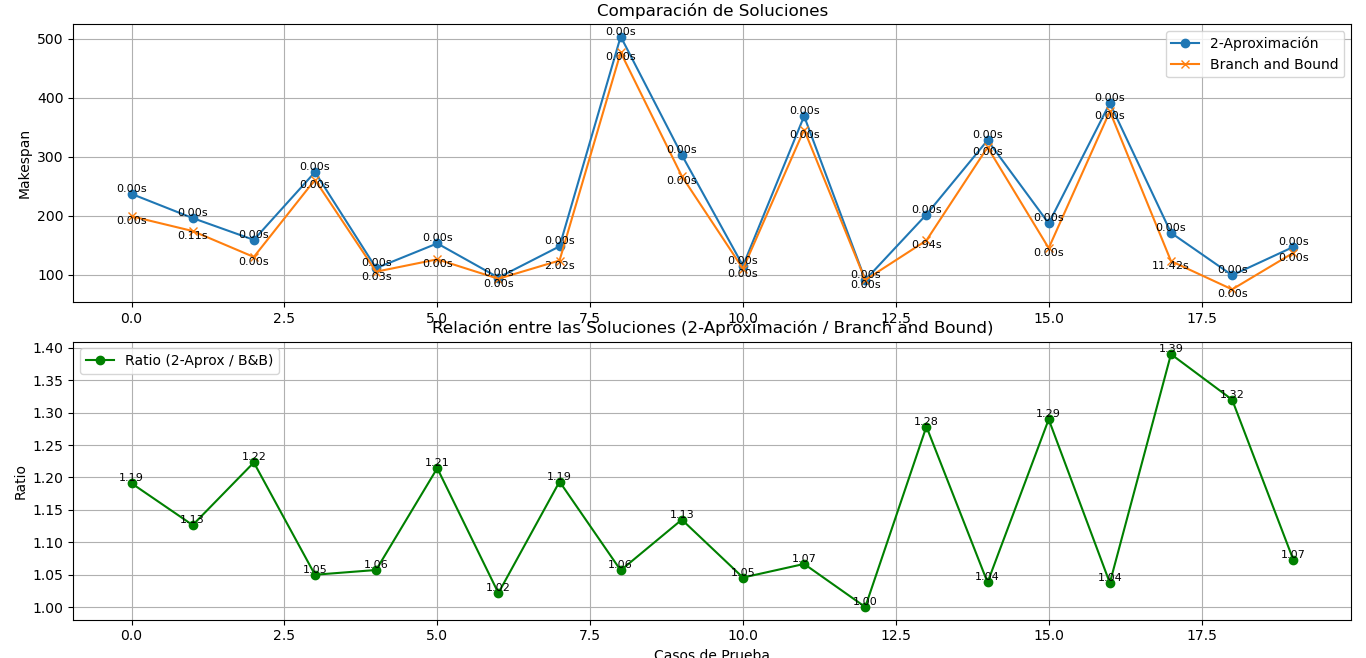
\includegraphics[width=1\linewidth]{Figure_1}
		\caption{Comparación gráfica entre los algoritmos}
		\label{fig:figure1}
	\end{figure}
	
	
	
	
	\begin{thebibliography}{9}
		
		\bibitem{CLRS2009}
		Thomas H. Cormen, Charles E. Leiserson, Ronald L. Rivest, and Clifford Stein.
		\textit{Introduction to Algorithms}.
		3rd ed. MIT Press, 2009.
		
		\bibitem{Rhee2016}
		Donguk Rhee.
		\textit{Esquemas de Aproximación Polinomial Más Rápidos para Problemas de la Mochila}.
		Tesis de Maestría en Investigación de Operaciones, Instituto Tecnológico de Massachusetts, 2016.
		
		\bibitem{Kleinberg2005}
		Jon Kleinberg and Éva Tardos.
		\textit{Algorithm Design}.
		1st ed. Pearson, 2005. Extraído de página 600.

		\bibitem{Garey1979}
		Michael R. Garey and David S. Johnson.
		\textit{Computers and Intractability: A Guide to the Theory of NP-Completeness}.
		1st ed. W. H. Freeman and Company, 1979.Extraído de página 238.
		
		
	\end{thebibliography}
\end{document}